\chapter{Media Item Compilation}
\label{cha:media-item-compilation}

% the code below specifies where the figures are stored
\ifpdf
    \graphicspath{{8_media_item_compilation/figures/PNG/}{8_media_item_compilation/figures/PDF/}{8_media_item_compilation/figures/}}
\else
    \graphicspath{{8_media_item_compilation/figures/EPS/}{8_media_item_compilation/figures/}}
\fi

\section{Introduction}

In this chapter, we introduce aesthetic principles
for the automatic generation of media galleries
based on media items retrieved from social networks
that---after a~ranking and pruning step---can serve to authentically
summarize events and their atmosphere from a~visual
and an audial standpoint.
Mobile devices such as smartphones, together with social networks,
enable people to create, share, and consume media items
like videos or photos.
They accompany their owners almost everywhere
and are thus omnipresent at all sorts of events.
Given a~stable network connection, event-related media items
and microposts are published on social networks
during events and afterwards.
Ranked media items stemming from multiple social networks
can serve to create authentic media galleries
that illustrate events and their atmosphere.
A~key feature for this task is the semantic enrichment
of media items and associated microposts
and the extraction of \emph{visual}, \emph{audial},
\emph{textual}, and \emph{social} features.
Based on this set of features,
additional \emph{aesthetic} features
can be defined and exploited to obtain appealing
and harmonic media galleries.

\begin{figure}[htb]
  \centering
  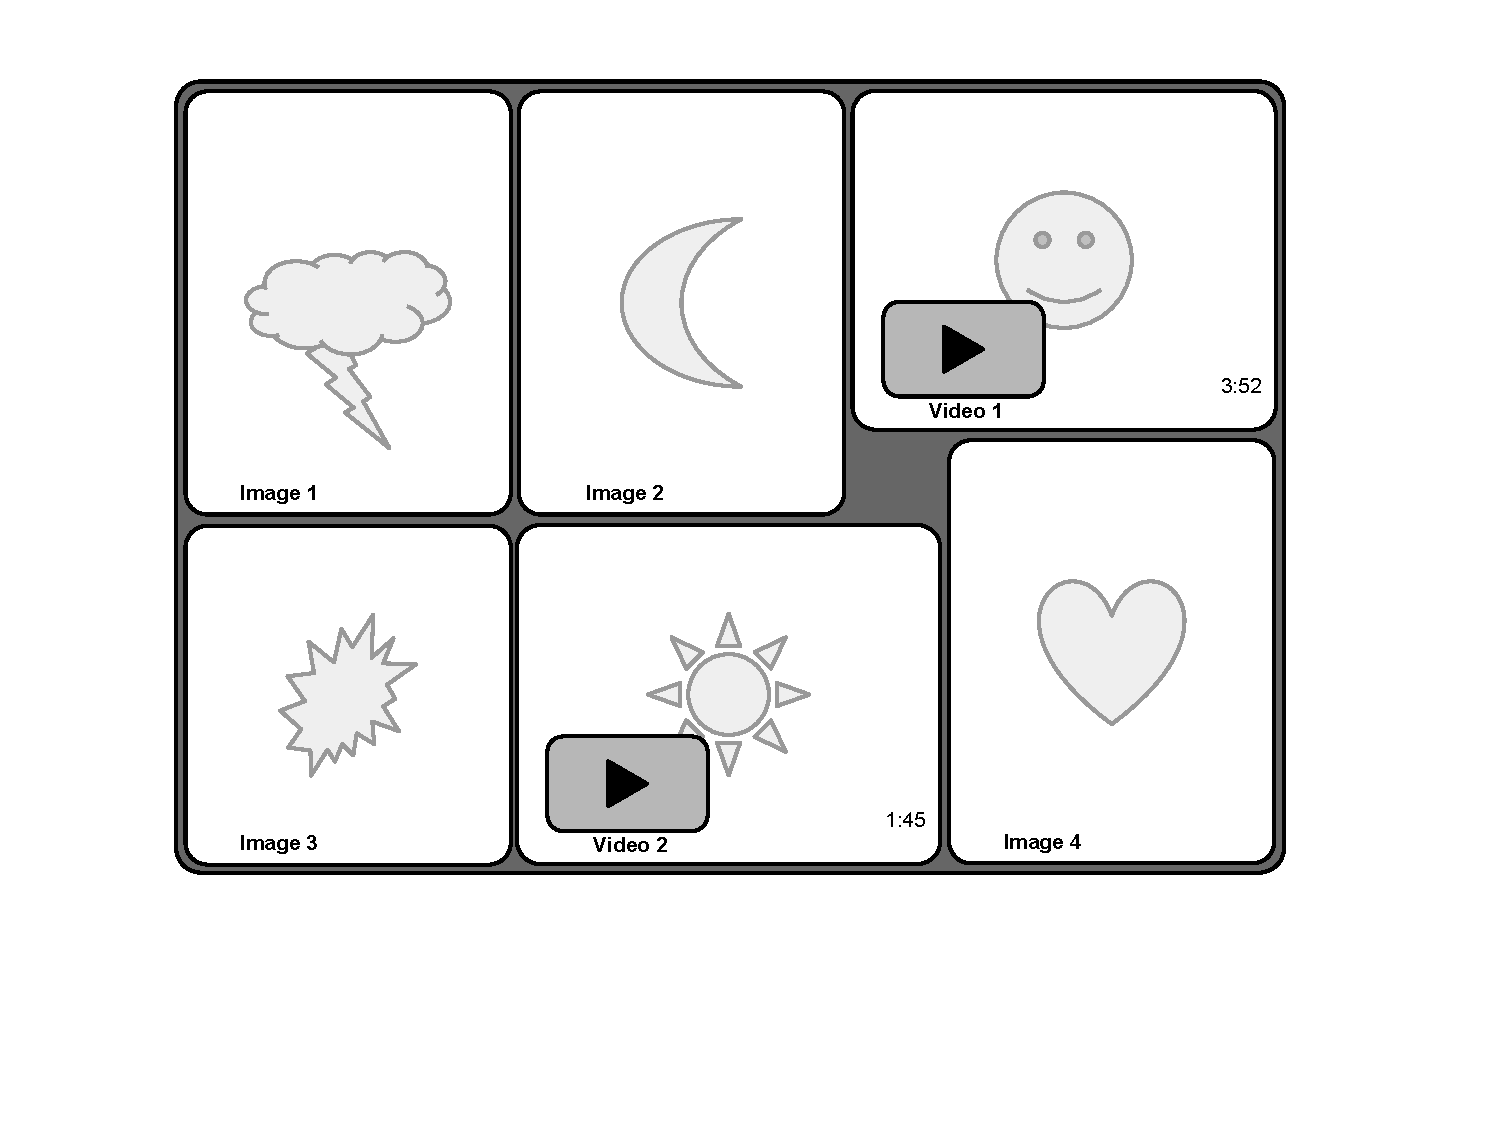
\includegraphics[trim=20mm 40mm 20mm 10mm, clip, width=0.7\columnwidth]{media-gallery.pdf}
  \caption{Schematic media gallery with four photos and two videos.}
  \label{fig:media-gallery}
\end{figure}

\section{Related Work}
While enormous efforts have been made to extract those features
from media items and microposts on social networks in \emph{isolation},
to the best of our knowledge, remarkably less initiatives 
concern the extraction and the application
of all those features \emph{in combination}
for \emph{all} types of media items, including microposts.
In~\cite{sandhaus2011photobook}, Sandhaus \emph{et al.}\ consider visual and
aesthetic features for the automatic creation of photo books.
Obrador \emph{et al.}\ use visual and aesthetic features
for a~category-based approach to automatically assess
the aesthetic appeal of photographs~\cite{obrador2012photoaesthetics}.
In~\cite{knees2006musicplaylist}, Knees \emph{et al.}\ use audial and textual
features for the automatic generation of music playlists.
Choudhury \emph{et al.}\ show in~\cite{choudhury2011sportstweets} how social and textual
features can be used to achieve precise detection results 
of named entities and significant events in sports-related microposts.
In~\cite{davidson2010videorecommendation}, Davidson \emph{et al.}\ show how visual,
textual, and social features can be used for personalized video recommendations.
A service called Storify~\cite{fincham2011storify} lets users manually combine
microposts, photos, videos, and other elements onto one page for the purpose
of storytelling or summarizing an event,
and share stories permanently on the Web.
Finally, social networks present photos and videos
often in grid-like galleries\footnote{\url{http://twitpic.com/904yka/full}},
sometimes scaled based on the amount of comments.
When unique media items have been collected,
the remaining task is to summarize events by selecting the most relevant media fragments. 
Fabro and B\"osz\"orm\'enyi~\cite{delfabro2012summarization} detail
the summarization and presentation of events from content retrieved from social media.
Nowadays, many domain-specific methods already exhibit good accuracy,
for example in the sports domain~\cite{li2001sportsvideo,li2010americanfootball}. However, the challenge is to find methods that are content-agnostic.
Methods that exploit semantic information~(\emph{e.g.},~\cite{chen2009videosummarization}) 
will likely provide high-quality results in the future,
but today's most relevant summaries are produced by user interaction~\cite{olsen2011videosummarization}.

\section{Media Gallery Aesthetics}

\noindent \textbf{Definition}
A media gallery is a~compilation of photos or videos
retrieved from social networks that are related to a~given event.
Given a~set $M = \{m_1,..., m_n\}$ of media items related to a~certain event,
a~ranking formula $f$, and a~ranking threshold $t$,
the subset $M^{\prime\prime} \subset M$
is the result after the application of $f$ to $M$: $f(M)=M^\prime$
and pruning the ranked set $M^\prime$ to only include members
whose rank is greater than $t$, with the resulting set named $M^{\prime\prime}$.
Each media item $m_i$ can either be an instance of a~video or photo.
For each point $t_x$ on a~timeline $T$, the state of the media gallery
at $t_x$ is defined for each media item $m_i$
as a~set $S_x$ of $n$ tuples $s_{x,i}$, where
$s_{x,i}=\langle \mathit{left}$, $\mathit{top}$, $\mathit{width}$, $\mathit{height}$,
$\mathit{alpha}$, $\mathit{z\mbox{-}index}$, $\mathit{animation}$,
$\mathit{start}$, $\mathit{playing}$, $\mathit{volume} \rangle$.
The first 6~properties are defined as in CSS, the $\mathit{animation}$ property
allows for the definition of CSS transitions
and transformations as defined in~\cite{CSSTransitions2009,CSSTransforms2012},
the $\mathit{start}$ property defines the start time in a~video.
A schematic media gallery at $t_x$ can be seen in \autoref{fig:media-gallery}.

\noindent \textbf{Audial aesthetics}
We recall the purpose of our media galleries:
to illustrate an event and its atmosphere.
Audial aesthetics thus consist of aspects like volume level normalization,
avoiding multiple videos playing music in parallel, smooth transitions, \emph{etc}.
We remark that through selective mixing of audio tracks
of event-related videos, ``noise clouds'' very characteristic
for the event atmosphere can be observed.

\noindent \textbf{Visual aesthetics}
Visual aesthetics are determined by the composition, \emph{i.e.},
the relation of the number of photos \emph{vs.} the number of videos \emph{globally},
\emph{per coherent scene}, and per \emph{point in time}.
In order to avoid cognitive overload of viewers,
the number of visible (moving) media items
at a~time should be limited.
Depending on the event, a~consistent or a~contrast-rich overall
appearance of items may be desired, also for transitions.

\section{Media Gallery Generation}

We have developed an application for the automatic generation of
media galleries that visually and audibly summarize events
based on media items like videos and photos from multiple social networks.
Further, we have evaluated different media gallery styles with online surveys 
and examined their advantages and disadvantages.
Besides the application itself,
where media galleries of different styles can be created on-the-fly,
our contributions are also the survey results.
A~demo is available at
\url{http://social-media-illustrator.herokuapp.com/}.

\section{Motivation}
\label{sec:motivation-chapter-8}

Media galleries (see \autoref{fig:media-gallery1} and \autoref{fig:media-gallery2}
for examples)
help users consume larger, however not overwhelmingly huge,
amounts of media items in an ideally pleasing and aesthetic way.
These media items may---or, more commonly: may not---be ordered,
besides an intrinsic chronologic order.
In the context of our work on summarizing events
based on microposts and media items stemming from
multiple social networks, we have created methods
to first \emph{extract} event-related media items
from multiple social networks, second, to
\emph{deduplicate} near- and exact-duplicate media items,
third, to \emph{cluster} them by visual similarity, and
finally, to \emph{rank} the resulting media item clusters
according to well-defined ranking criteria.
In this chapter, we treat the challenge of \emph{compiling}
ranked media item clusters in media galleries in ways
such that the ranking-implied order is (loosely) respected.
In the previous sections, we have defined
aesthetic principles for automatic media gallery layout~\cite{steiner2012definingaesthetic},
which we now apply to media gallery styles.
The task of media gallery compilation is different
from the widely researched task of photo book generation,
as media galleries can contain both, photos and videos.
Different types of media gallery layouts are possible,
two of which we have implemented and evaluated via two different user studies.
One with, and one without detailed user comments.

\section{Media Gallery Styles}

Media galleries---in contrast to free-form digital media collages---%
necessarily display media items in a~grid-like way.
The crucial question is thus whether the media items' aspect ratios
should be respected, or whether they should be cropped to square,
or other aspect ratios (\emph{e.g.}, 4:3 or 16:9).
Respecting the aspect ratio has the advantage that media items
do not need to be potentially lossily cropped,
however, due to the unpredictable media item formats,
compiling media galleries that do not look frayed is harder.
The advantage of cropping is that media gallery layout is easier,
as the media item formats are predictably the same,
at the cost of having to decide where to crop.
Different algorithms (\emph{e.g.},~\cite{suh2003thumbnail})
beyond this chapter's scope exist to aid this decision.
A~media gallery is called \emph{balanced}, if its shape is rectangular,
\emph{hole-free} if there are no gaps from missing media items,
and \emph{order-respecting},
if media items appear in insertion order.

\paragraph{Non-Order-Respecting Styles}

An interesting technique for arranging media items is dividing.
Paper sizes that follow the ISO~216 standard%
\footnote{\url{http://www.iso.org/iso/iso_catalogue/catalogue_tc/catalogue_detail.htm?csnumber=36631},
accessed March 27, 2013}
are the most common every-day examples of the dividing principle:
every media item with an aspect ratio of $ \sqrt2 $ can be divided
into two media items with the same aspect ratio.%
\footnote{\url{http://blog.vjeux.com/2012/image/image-layout-algorithm-lightbox-android.html},
as~of 02/22/2013}
This works for portrait and landscape orientations,
however, is not necessarily order-respecting.
Two other non-order-respecting techniques are (i),~%
working with pre-defined placeholder patterns
(small and big squares, portrait and landscape rectangles)
and then filling the placeholder shapes with media items,%
\footnote{\url{http://blog.vjeux.com/2012/image/image-layout-algorithm-500px.html},
as~of 02/22/2013}
or (ii),~working with columns of pre-defined widths
and then iteratively inserting in the smallest column.%
\footnote{\url{http://blog.vjeux.com/2012/image/image-layout-algorithm-lightbox.html},
as~of 02/22/2013}
As outlined in \autoref{sec:motivation-chapter-8},
we require (at least loosely) order-respecting media galleries
for the ranking step to make sense.
In the upcoming two subsections, we will introduce two techniques
for the generation of such media galleries.

\paragraph{Strict Order, Equal Size (SOES)}

A~media gallery style that we call \emph{Strict Order, Equal Size (SOES)},
which strictly respects the ranking-implied order is presented in~%
\cite{chedeau2012googleplus}.
Examples can be seen in \autoref{fig:a} and \autoref{fig:c}.
The algorithm works by resizing all media items in a~row to the same height
and adjusting the widths in a~way that the aspect ratios are maintained.
A~row is filled until a~maximum row height is reached,
then a~new row (with potentially different height) starts, \emph{etc.}
This media gallery style is order-respecting, hole-free,
and can be balanced by adjusting the number
of media items in $+1$ steps.

\begin{figure}[t!]
  \centering
  \subfloat[\emph{SOES}, Survey~A]{
    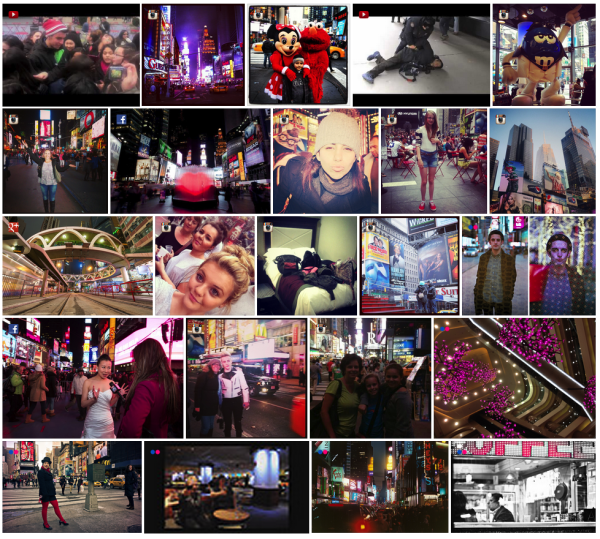
\includegraphics[height=5cm]{equal-size.png}
    \label{fig:a}
  }                
  \subfloat[\emph{LOVS}, Survey~A]{
    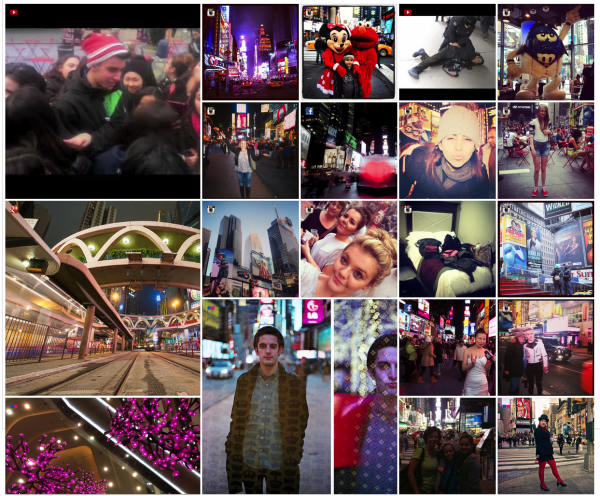
\includegraphics[height=5cm]{different-size.png}
    \label{fig:b}
  }
  \caption{Survey~A: Media galleries visualizing a~gathering at Times Square, New York on February 8, 2013}
  \label{fig:media-gallery1}  
\end{figure}

\begin{figure}[t!]
  \centering
  \subfloat[\emph{SOES}, Survey~B]{
    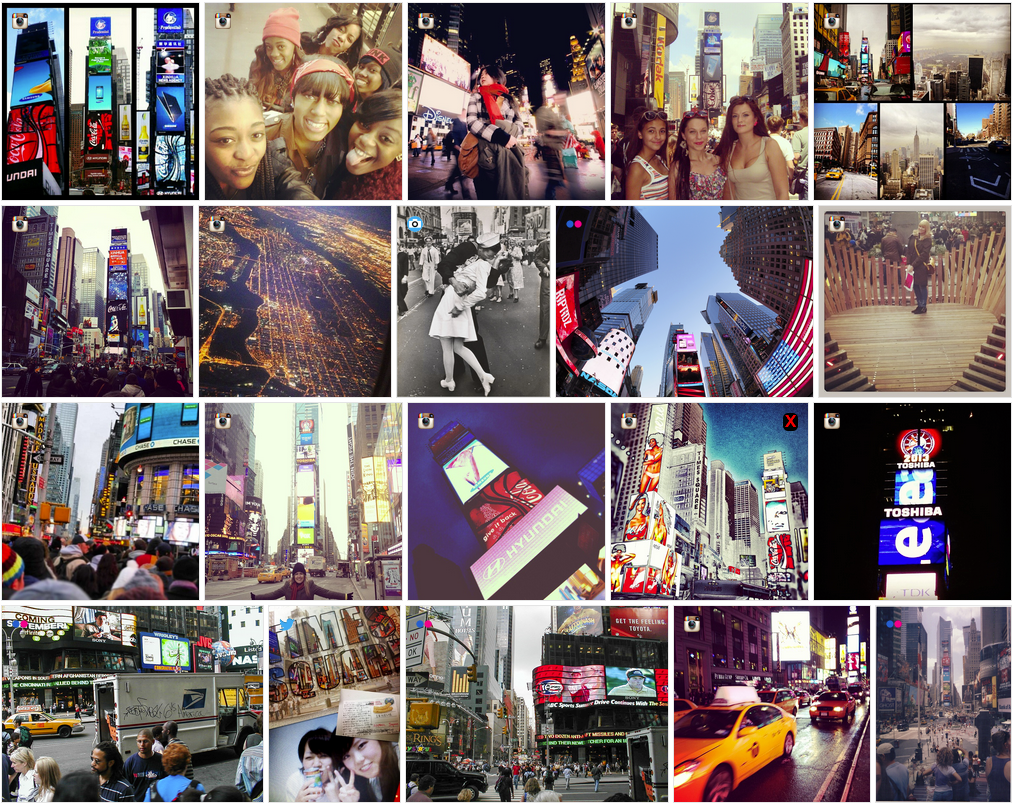
\includegraphics[height=5cm]{timessquare_2.png}
    \label{fig:c}
  }                
  \subfloat[\emph{LOVS}, Survey~B]{
    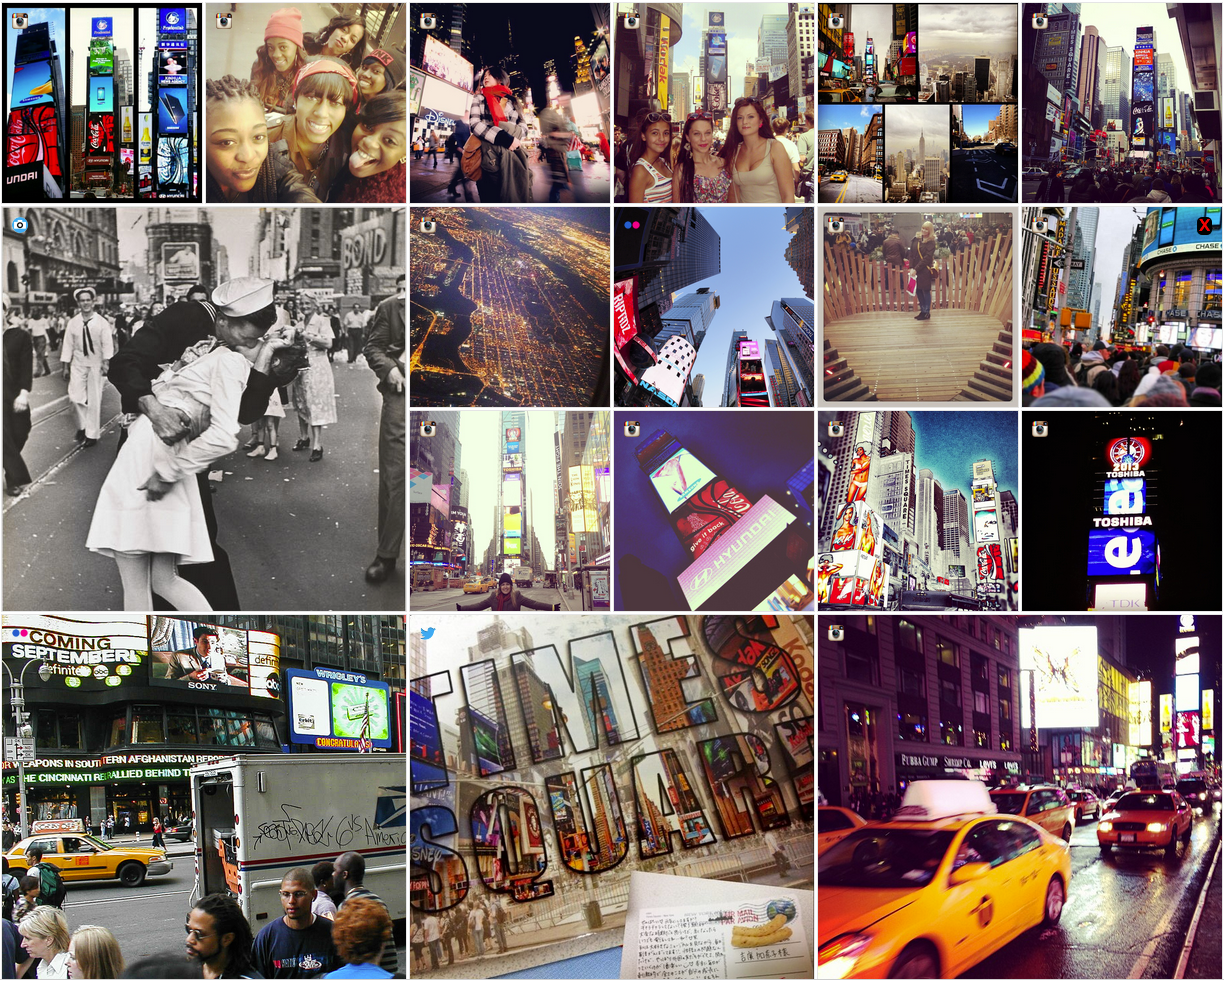
\includegraphics[height=5cm]{timessquare_1.png}
    \label{fig:d}
  }
  \caption{Survey~B: Media galleries visualizing a~gathering at Times Square, New York on February 8, 2013}
  \label{fig:media-gallery2}  
\end{figure}

\paragraph{Loose Order, Varying Size (LOVS)}

Examples of a~media gallery style
that we call \emph{Loose Order, Varying Size (LOVS)}
can be seen in \autoref{fig:b} and \autoref{fig:d},
with the details explained in~\cite{chedeau2012facebook}.
The algorithm works by cropping all images to a~square aspect ratio,
which allows for organizing media items such that one big square always
contains two horizontal blocks, each with two pairs of small squares.
The media gallery is then formed by iteratively filling
big or small squares until a~square is full,
and then adding it to the smallest column.
This media gallery style allows any media item to become big,
while still being loosely order-respecting and always hole-free.
Balancing the gallery is slightly harder,
as in the worst case up to $ (\mathit{bigBlocksPerRow} - 1) \times 2 $
media items may be required.

\section{Discussion and Evaluation}

The main motivation for the \emph{Loose Order, Varying Size} style
is that certain media items can be featured more prominently
by making them big, while still loosely respecting the ranking-implied order.
Examples of to-be-featured media items can be videos,
media items with faces, media items available in High-Density quality,
or media items with interesting details~%
\cite{suh2003thumbnail}.
Users may want to decide what media items to feature,
albeit we aim for an automatized solution.
Evaluating subjective data like \emph{the} correct presentation form
for a~set of media items is a~challenging task.
For different users and different media galleries,
there may be different optimal settings.
A~common subjective evaluation technique
is the Mean~Opinion Score (MOS),
used for decades in telephony networks to
obtain the human user's view of the quality of a~network.%
\footnote{\url{http://www.itu.int/rec/T-REC-P.800-199608-I/en},
as~of 02/21/2013}
Recently, MOS has also found wider usage in the multimedia community.
Therefore, a~set of standard subjective tests are conducted,
where users rate the perceived quality of test samples
with scores from 1 (worst) to 5 (best).
The actual MOS is then the arithmetic mean of all individual scores.

We have conducted two types of surveys. 
Survey~A via multiple social networks, where we simply asked people to ``Like''
and/or comment on their favorite style of media gallery,
and Survey~B via email to a~company-internal ``miscellaneous'' mailing list,
where we asked people to rate media galleries via MOS, with optional comments. 
Survey~A and Survey~B used different media items in the media galleries,
as to have some measure in how far content has an impact.

For Survey~A on the social networks Twitter, Facebook,
and \googleplus, we had overall 16~participants (7~female, 8~male, 1~unknown).
7~users liked \emph{SOES} more,
whereas 9~users liked \emph{LOVS} more.
Interestingly, no user commented on why they liked \emph{SOES} more.
Users who commented on why they liked \emph{LOVS} more mentioned
they liked the additional structure and tidiness,
the fact that some media items were bigger,
the fact that it was easier to identify individual media items,
and the fact that important media items were highlighted.

For Survey~B via email with MOS ratings,
we had 19~participants (6~female, 13~male).
The majority of users who liked \emph{LOVS} more
mentioned that the different sizes
gave the eye focal points and orientation,
whereas one user explicitly disliked this guidance.
Users liked the harmony and the structure.
Two users mentioned that small media items were proportionally too small.
Regarding \emph{SOES}, users reported they felt overloaded
and did not know where to start.
Some users said the layout was boring and that,
while they liked the outer framing,
they were confused by the irregular inner grid.
The MOS for \emph{SOES} was $2.39$ (variance $0.68$),
the MOS for \emph{LOVS} was $4.17$ (variance $0.47$).
The data of Survey~B is available.%
\footnote{\url{http://bit.ly/media-gallery-survey},
as~of 02/22/2013}

\section{Conclusions and Future Work}

We have created an application that auto-generates 
two media gallery styles, \emph{SOES} and \emph{LOVS},
and evaluated users' perceived quality with two separate surveys. 
While the data is not significant, the trend is that users
seem to prefer \emph{LOVS}.
Future work will be on evaluating more media gallery styles.
Concluding, we have learned that eyes need focal points
to spot the needles in the media gallery haystack.

\section*{Chapter Notes}
This chapter is partly based on the following publications:
\todo{Add publications}